

%\section{État de l'art}
\section{Méthodes de projection de liquides}
\subsection{Bombe spray}
Pour constituer des écrans de turbulence aisément, l'approche de la bombe de spray pour les cheveux
, ou de laque transparente pour surfaces a été employée.
\begin{figure}[H]
    \centering
    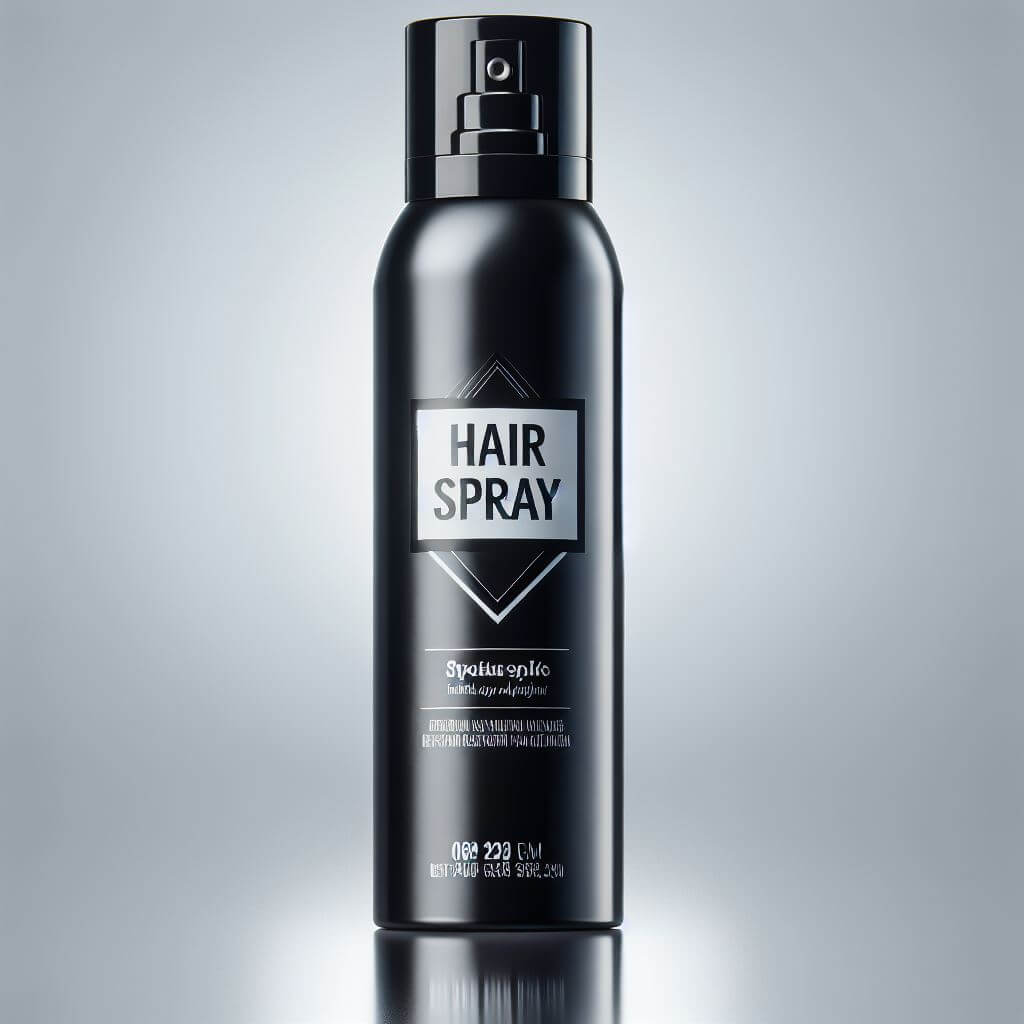
\includegraphics[width=0.3\textwidth,trim={4cm 0 4cm 0},clip]{assets/figures/etat_art/airspray.jpeg}

    \caption{Bombe de laque (IA)}
\end{figure}
Cette solution étant assez sommaire et peu reproductible, elle a été abandonnée au profit de méthodes plus contrôlables.
La durée du "pschit" est sujette à l'erreur humaine, la quantité de liquide projetée
dépend directement de la durée d'appui mais aussi de la pression du gaz de la bombe, cette
dernière diminuant au fil des usages et variant en fonction de la température et de l'altitude,
explique pourquoi cette solution ne fut pas sélectionnée.

% Please add the following required packages to your document preamble:
% \usepackage[table,xcdraw]{xcolor}
% Beamer presentation requires \usepackage{colortbl} instead of \usepackage[table,xcdraw]{xcolor}
\begin{table}[H]
    \centering
    \begin{tabular}{|c|c|lll}
        \cline{1-2}
        Avantages                                 & Inconvénients                                                          &  &  & \\ \cline{1-2}
        \cellcolor[HTML]{67FD9A}Abordable         & \cellcolor[HTML]{FD6864}Durée de "pschit" hasardeuse                   &  &  & \\ \cline{1-2}
        \cellcolor[HTML]{67FD9A}trouvable partout & \cellcolor[HTML]{FD6864}Dépendante de la température et de la pression &  &  & \\ \cline{1-2}
                                                  & \cellcolor[HTML]{FD6864}Très artisanal                                 &  &  & \\ \cline{1-2}
    \end{tabular}
    \caption{Résumé des avantages et inconvénients du spray}
    \label{tab:hair_spray_table}
\end{table}

\newpage
\subsection{Aérographe} \label{section_aerographe}
L'aérographe est un pistolet à peinture miniature similaire à un pistolet généralement utilisé pour les traveaux de précision
à peinture utilisé par les carrossiers.
Ces derniers sont généralement alimentés à l'aide d'un compresseur et peuvent projeter plusieurs médiums.

\begin{figure}[H]
    \centering
    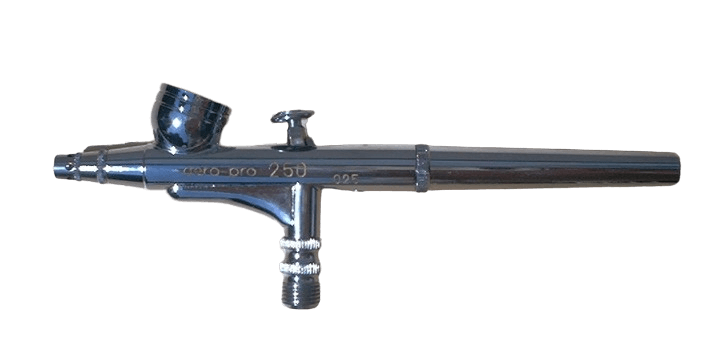
\includegraphics[width=0.8\textwidth]{assets/figures/etat_art/airbrush.png}
    \caption[Aérographe]{Aérographe \cite{airbrush_pics}\footnotemark}
\end{figure}
\footnotetext{\url{http://ingo-karkat.de/textilepainting/About\%20used\%20tools/index.html}}

L'aérographe repose sur l'effet venturi, l'air comprimé entraine le liquide à projeter dans l'embouchure assez fine de l'outil
transformant ce dernier en goutelettes plus ou moins fines en fonction du réglage de l'aiguille de l'outil.

\begin{figure}[H]
    \centering
    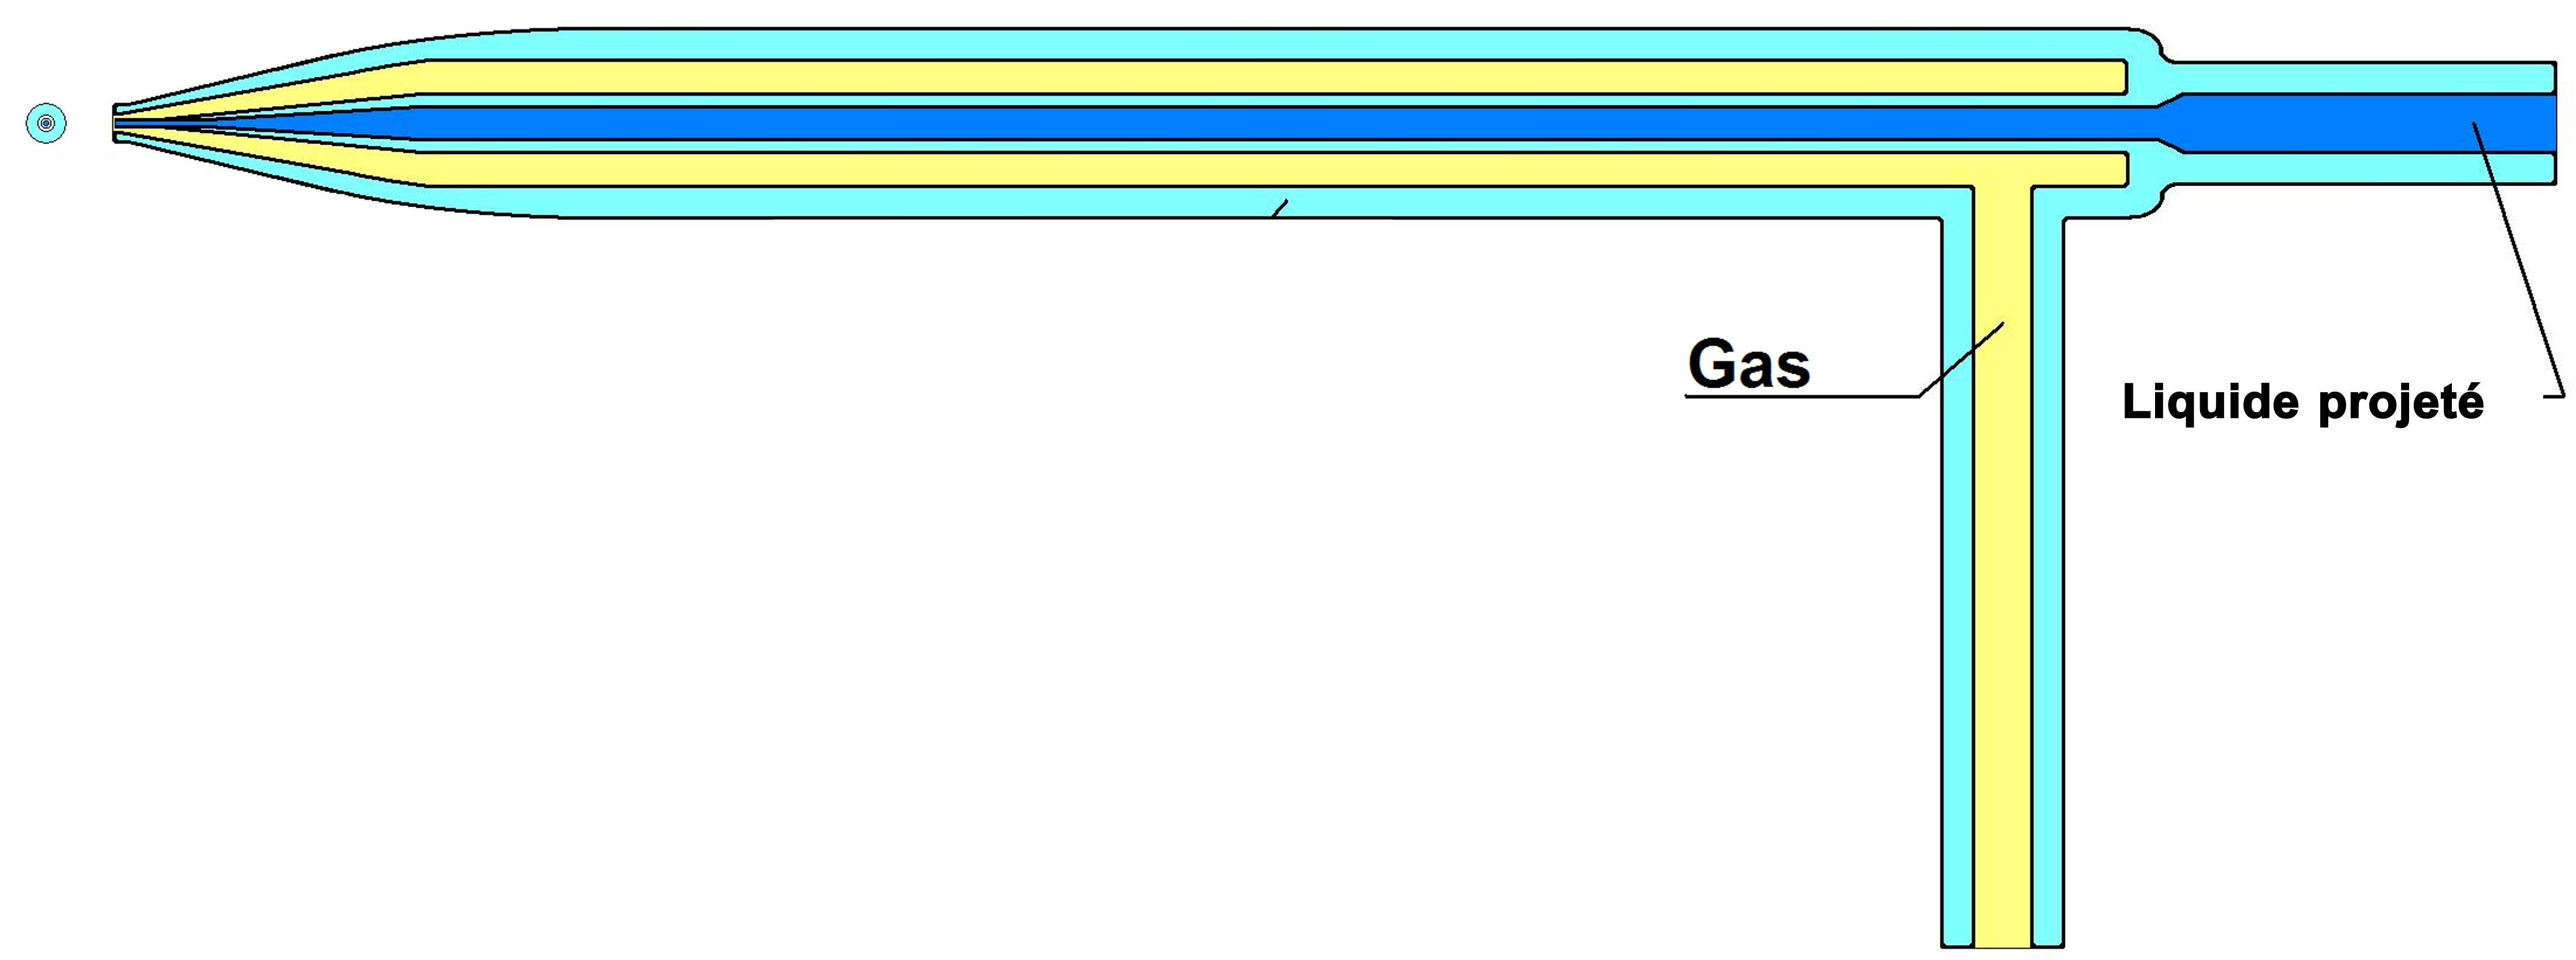
\includegraphics[width=0.6\textwidth]{assets/figures/etat_art/effet_venturi_aerographe.jpg}
    \caption[Effet venturi dans aérographe]{Effet venturi dans aérographe \cite{venturi_airbrush}\footnotemark}
\end{figure}
\footnotetext{\url{https://upload.wikimedia.org/wikipedia/commons/1/1e/Nebulizzatoe\_concentrico.png}}

C'est la solution de projection selectionnée dans la machine actuelle, il a pour avantage, d'être réglable assez finement
et de ne nécessiter qu'un compresseur, le critère de selection principal lors du choix effectué par le concepteur de la machine
était la disponibilité de l'outil de façon rapide en l'empruntant à un tier.

% Please add the following required packages to your document preamble:
% \usepackage[table,xcdraw]{xcolor}
% Beamer presentation requires \usepackage{colortbl} instead of \usepackage[table,xcdraw]{xcolor}
\begin{table}[H]
    \centering
    \begin{tabular}{|c|c|lll}
        \cline{1-2}
        Avantages                                                                                            & Inconvénients                                     &  &  & \\ \cline{1-2}
        \cellcolor[HTML]{67FD9A}Non influencé par l'environnement                                            & \cellcolor[HTML]{FD6864}Montage actuel capricieux &  &  & \\ \cline{1-2}
        \cellcolor[HTML]{67FD9A}Motorisable -\textgreater reproductible                                      & \cellcolor[HTML]{FFFFFF}                          &  &  & \\ \cline{1-2}
        \cellcolor[HTML]{67FD9A}Beaucoup de possibilités de modifier la brumisation                          & \cellcolor[HTML]{FFFFFF}                          &  &  & \\ \cline{1-2}
        \multicolumn{1}{|l|}{\cellcolor[HTML]{67FD9A}Possibilité de contrôler la composition de l'acrylique} & \multicolumn{1}{l|}{}                             &  &  & \\ \cline{1-2}
        \multicolumn{1}{|l|}{\cellcolor[HTML]{67FD9A}Bouton qui bloque l'air intégré}                        & \multicolumn{1}{l|}{}                             &  &  & \\ \cline{1-2}
    \end{tabular}
    \caption{Résumé des avantages et inconvénients de l'aérographe}
    \label{tab:aerographe_table}
\end{table}
\subsection{Atomiseurs pneumatiques}
Les atomiseurs pneumatiques reposent sur le même principe de fonctionnement que l'aérographe de la \autoref{section_aerographe}, donc avec effet
venturi et une aiguille pour régler la taille des goutelettes.
\begin{figure}[H]
    \centering
    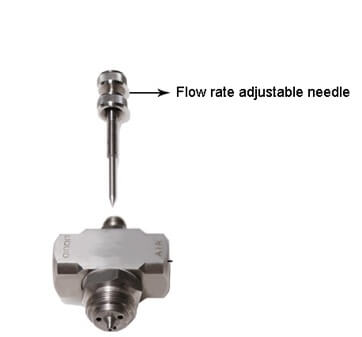
\includegraphics[width=0.5\textwidth]{assets/figures/etat_art/atomizing_nozzle.jpg}
    \caption[Buse d'atomisation pneumatique]{Buse d'atomisation pneumatique \autocite{photo_buse_atomisation}\footnotemark}
\end{figure}
\footnotetext{\url{https://www.nozzlespray.com/uploads/allimg/220310/atomizingfogspraynozzlefordisinfection.jpg}}

Ces buses d'atomisation à air comprimé sont utilisées dans l'industrie pour recouvrir des surfaces (peinture), nettoyer avec de l'eau, dans la confection d'aliments et bien d'autre:
\begin{figure}[H]
    \centering
    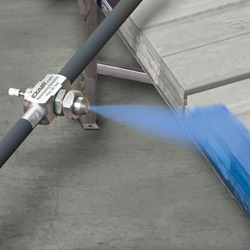
\includegraphics[width=0.5\textwidth]{assets/figures/etat_art/buse spray.jpeg}
    \caption[Exemple d'application d'une buse d'atomisation]{Exemple d'application d'une buse d'atomisation \autocite{exemple_application_buse}\footnotemark}
\end{figure}
\footnotetext{\url{https://english.exair.com/images/atom/IntMix-2\_250sq.png}}
\newpage
Elles permettent un choix de formes de projection assez vaste :
\begin{figure}[H]
    \centering
    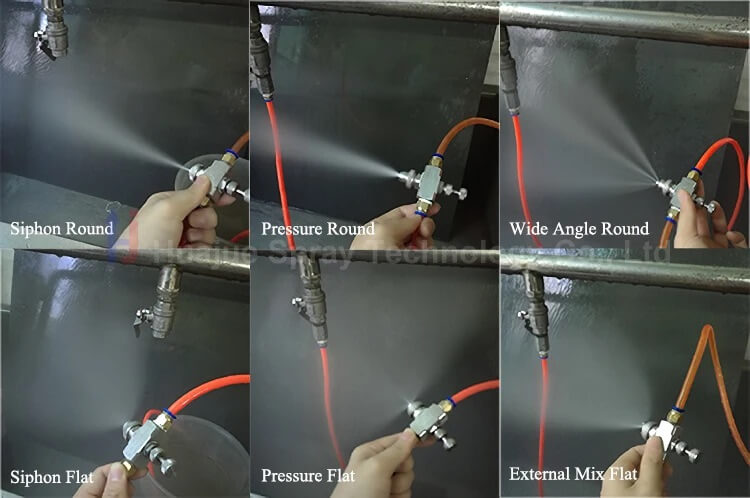
\includegraphics[width=0.9\textwidth]{assets/figures/etat_art/spray_patterns_example.jpeg}
    \caption[Exemples de différents "motifs" de spray]{Exemples de différents "motifs" de spray \autocite{Exemples_spray_patterns}\footnotemark}
\end{figure}
\footnotetext{\url{https://ae01.alicdn.com/kf/H428bb75251884fee8f19beffbbd38cfdp.jpg}}
C'est une piste de solution intéressante, elle fait déjà ses preuves dans plusieurs industries différentes.
L'activation du spray devra se faire de façon externe avec une electrovanne par exemple. Concernant la gestion de la taille
des goutelettes il faudra automatiser l'actionnement de l'aiguille. Concernant un point important pour ce type de matériel industriel est le prix,
des fournisseurs chinois pratiqueront des prix dans l'ordre de 10-20 frs, tandis que des fournisseurs traditionnels se situent plus dans les 300-800 frs. Il n'y semble
pas y avoir de milieu de gamme.

% Please add the following required packages to your document preamble:
% \usepackage{graphicx}
% \usepackage[table,xcdraw]{xcolor}
% Beamer presentation requires \usepackage{colortbl} instead of \usepackage[table,xcdraw]{xcolor}
\begin{table}[H]
    \centering
    \resizebox{\textwidth}{!}{%
        \begin{tabular}{|c|c|lll}
            \cline{1-2}
            Avantages                                                                                            & Inconvénients                                                  &  &  & \\ \cline{1-2}
            \cellcolor[HTML]{67FD9A}Non influencé par l'environnement                                            & \cellcolor[HTML]{FD6864}Pas de bouton de blocage du flux d'air &  &  & \\ \cline{1-2}
            \cellcolor[HTML]{67FD9A}Motorisable -\textgreater reproductible                                      & \cellcolor[HTML]{FD6864}Classes de prix non régulières         &  &  & \\ \cline{1-2}
            \cellcolor[HTML]{67FD9A}Beaucoup de possibilités de modifier la brumisation                          & \cellcolor[HTML]{FFFFFF}                                       &  &  & \\ \cline{1-2}
            \multicolumn{1}{|l|}{\cellcolor[HTML]{67FD9A}Possibilité de contrôler la composition de l'acrylique} & \multicolumn{1}{l|}{}                                          &  &  & \\ \cline{1-2}
            \multicolumn{1}{|l|}{\cellcolor[HTML]{67FD9A}Solution utilisée dans l'industrie}                     & \multicolumn{1}{l|}{}                                          &  &  & \\ \cline{1-2}
            \multicolumn{1}{|l|}{\cellcolor[HTML]{67FD9A}Méthode de montage standardisée}                        & \multicolumn{1}{l|}{}                                          &  &  & \\ \cline{1-2}
        \end{tabular}%
    }
    \caption{Résumé des avantages et inconvénients de l'atomiseur pneumatique}
    \label{tab:atomiseur_pneumatique_table}
\end{table}
